%% FSE 2027 draft — leakage-controlled agentic RCA over four telemetry modalities
%% Build: latexmk -pdf main.tex   (requires ACM acmart class)
%% For submission switch to:  \documentclass[sigconf,review,anonymous]{acmart}
\documentclass[sigconf]{acmart}

\usepackage{booktabs}
\usepackage{xspace}
\usepackage{pgfplots}
\pgfplotsset{compat=1.17}

%% ---- draft helpers (strip before submission) ----------------------------------------
\newcommand{\todo}[1]{\textcolor{red}{\textbf{[TODO: #1]}}}
\newcommand{\sys}{StrataTrace\xspace}
\newcommand{\agent}{the agent\xspace}

%% ---- ACM metadata (TODO before submission) ------------------------------------------
\setcopyright{none}
\acmConference[FSE 2027]{ACM International Conference on the Foundations of Software
Engineering}{TBD 2027}{TBD}
\acmDOI{}
\acmISBN{}

\begin{document}

\title{How Much Observability Does an LLM Agent Need?\\
Leakage-Controlled Root-Cause Analysis over Four Telemetry Modalities}
%% Alt titles:
%% Honest Agents: Quantifying and Eliminating Evaluation Leakage in LLM-Based RCA
%% Kernel Deep, Trace Thin: Stress-Testing an LLM RCA Agent's Observability Diet

\author{Yuvraj Sehgal}
\affiliation{\institution{\todo{affiliation}}\country{Canada}}
\email{17yuvraj.sehgal@gmail.com}
%% \author{...} \todo{co-authors, order}

\begin{abstract}
LLM agents are rapidly being adopted for root-cause analysis (RCA) in microservice
systems, but their reported accuracy is difficult to trust: benchmark artifacts ---
fault-encoding run identifiers, injection containers named after their faults --- hand
the agent the answer. We present a leakage-controlled evaluation methodology (identifier
masking with cross-tool identity preservation, full-fidelity audit transcripts, and an
automated leak auditor) and apply it to a new dataset: 95 labeled fault injections
across two architecturally distinct microservice systems, recorded simultaneously in
\emph{four} time-aligned telemetry modalities --- metrics, logs, distributed traces,
and \emph{kernel traces} --- with pre-registered fault$\rightarrow$modality predictions.
We find that naming leaks alone inflate an agent's fault-classification accuracy by
57~percentage points; after closing them, a tool-using agent with generic
cross-modality tooling still reaches 83--87\% top-1 service localization, roughly
double two non-LLM baselines including published state of the art, at ${\sim}\$0.01$
per incident. Degradation experiments yield three counter-intuitive results: accuracy
survives $20\times$ trace sampling unchanged; removing kernel telemetry entirely costs
little accuracy but 34\% more investigation effort; and a \emph{partial} kernel view
(raw KPIs without interpretive framing) is \emph{worse than none}. An experience layer
of reusable ``skills'' helps only when skill selection is reliable --- mis-selected
skills cost more than they contribute. All 500+ diagnoses ship with machine-checkable
no-leakage certificates. \todo{tighten to venue word limit}
\end{abstract}

%% TODO: CCS concepts + keywords (required by acmart)
\begin{CCSXML}
<ccs2012>
<concept><concept_id>10011007.10011074.10011099</concept_id>
<concept_desc>Software and its engineering~Software verification and validation</concept_desc>
<concept_significance>500</concept_significance></concept>
</ccs2012>
\end{CCSXML}
\ccsdesc[500]{Software and its engineering~Software verification and validation}
\keywords{root-cause analysis, LLM agents, observability, kernel tracing, benchmark
leakage, microservices, AIOps}


\maketitle

\section{Introduction}
\label{sec:intro}

Automated root-cause analysis (RCA) for microservice incidents directly affects
time-to-mitigation, and LLM-based agents are the current frontier: they read
heterogeneous telemetry, form hypotheses, drive diagnostic tools, and explain their
conclusions. But an uncomfortable question precedes any accuracy claim for such agents:
\emph{did the agent diagnose the fault, or read the answer off the benchmark?}
Injected-fault datasets --- including ours, initially --- encode their labels
everywhere: run identifiers such as \texttt{tt\_slow\_db\_aggressive\_steady\_r1},
injection containers named \texttt{noisy-neighbor}, metric fields named
\texttt{injection}. A language model that sees any of these needs no telemetry at all.

\paragraph{What we did.} We built (i) \sys, a two-application, four-modality incident
dataset whose kernel-trace layer no existing public dataset provides; (ii) a tool-using
LLM RCA agent operating over deterministic, byte-accounted telemetry tools; and (iii) a
leakage-control harness --- masking, full-fidelity transcripts, and an automated audit
--- that lets us report, to our knowledge for the first time, \emph{certified
hint-free} agent RCA numbers, together with the exact price of the hints we removed.

\paragraph{The evaluation arc is itself a finding.} Our agent initially scored
74/74/61 (service / fault-type / both correct). Closing the leaks collapsed it to
48/17/9 --- proof that it had been leaning on names. Rebuilding the agent with strictly
generic tooling (baseline-vs-incident discipline in every tool, call-graph topology
with peer edges, host and limit-proximity channels, fault-taxonomy definitions)
recovered 83/48/48 --- \emph{above} the leaky number on localization, with every crutch
removed. The sequence quantifies both the contamination risk (26~points of service
accuracy, 57~points of fault classification) and its recoverability by honest means.

\paragraph{Contributions.}
\begin{enumerate}
  \item \textbf{Methodology.} Leakage-controlled agent evaluation: evidence-preserving
  identifier masking (with a cross-tool identity requirement --- masking must not
  fragment one entity into several pseudonyms), ground-truth-free audit transcripts, an
  automated leak auditor, and an A/A variance protocol that bounds single-run claims
  ($\pm$9 points in our setting).
  \item \textbf{Dataset and system.} \sys: 95 labeled runs over Sock~Shop and
  Train-Ticket, four time-aligned modalities (${\sim}0.001$\,ms clock skew), a kernel
  representation ladder (raw CTF $\rightarrow$ per-second KPIs $\rightarrow$ wait
  attribution $\rightarrow$ natural-language digests), pre-registered
  fault$\rightarrow$modality predictions; plus an open agentic-RCA harness with two
  non-LLM baselines and a published state-of-the-art adapter.
  \item \textbf{Empirical results.} (a)~The leak-free agent roughly doubles non-LLM
  baselines on top-1 service localization; (b)~accuracy shows \emph{no cliff} down to
  5\% trace sampling --- traces are ${\sim}20\times$ over-collected for this task;
  (c)~kernel telemetry buys efficiency ($-25$\% agent effort) and induced-DB-latency
  \emph{typing}, while its accuracy-rescue role is absorbed by good cross-modality
  tooling; (d)~\emph{interpreted} kernel summaries beat raw KPIs --- a partial kernel
  view degrades below kernel-blind; (e)~an experience/skill layer is net-negative
  without reliable evidence-based skill selection; unseen-fault incidents under a full
  skill library cost ${\sim}18$ points (a quantified distractor effect, via
  leave-one-family-out).
\end{enumerate}

\todo{one-paragraph roadmap of the paper}

\section{Background and Related Work}
\label{sec:background}

\paragraph{Non-LLM RCA.} Statistical and spectrum-based localization over metrics and
traces is well studied; we compare against a hand-built statistical rule tree and the
RCAEval/BARO family~\cite{pham2024baro,pham2025rcaeval}, whose artifacts we run
directly, plus the trace-only methods MicroRank~\cite{yu2021microrank} and
TraceRCA~\cite{li2021tracerca}. \todo{verify citations; add spectrum-based and
causal-discovery lines}

\paragraph{LLM and agentic AIOps.} Recent systems apply LLMs to incident triage and
RCA \todo{cite RCACopilot, HolmesGPT, mABC, and 2025--2026 agentic RCA papers}. To our
knowledge none report leakage-controlled numbers; evaluations typically expose
dataset-native identifiers to the model.

\paragraph{Benchmark contamination.} Label leakage and contamination are recognized
threats in ML evaluation \todo{cite contamination literature}; we bring this discipline
to agentic AIOps, where the leak channels are structural (identifiers in telemetry)
rather than train/test overlap.

\paragraph{Observability datasets.} Public microservice incident datasets
\todo{cite Train-Ticket fault studies \cite{zhou2018trainticket}, RCAEval datasets,
Nezha, AIOps challenge corpora} provide metrics/logs/traces; none include synchronized
kernel traces, and none pre-register per-fault modality predictions.

\paragraph{Kernel tracing.} LTTng~\cite{desnoyers2006lttng} provides low-overhead
full-syscall tracing; eBPF-based diagnosis is adjacent \todo{cite}. Our measured
collection overhead is $-0.5$\% throughput and $+12.6$\% P95 latency at 200 concurrent
users.

\section{The \sys{} Dataset}
\label{sec:dataset}

\paragraph{Subjects.} Two systems chosen for architectural contrast.
\emph{Sock~Shop}: 14 services, one datastore per service, and deliberately partial
trace instrumentation (6/14 services emit spans; trace blind spots are a design
variable, recorded per fault as \texttt{target\_trace\_visibility}).
\emph{Train-Ticket}~\cite{zhou2018trainticket}: ${\sim}40$ Java services sharing one
MySQL instance --- a structurally trace-blind choke point through which every service's
queries flow.

\paragraph{Faults.} Twelve fault types in five families: host resource exhaustion
(CPU, disk, memory, network), per-service resource caps (CPU throttle, memory limit),
application faults (induced database latency via an always-in-path proxy; connection
error storms), dependency faults (frozen dependency; silent asynchronous queue
backlog), and infrastructure faults (noisy neighbor; per-service network degradation).
Each recipe writes machine-readable ground truth (target, window, expected blast
radius) and an independent verification verdict.

\paragraph{Runs and alignment.} Each run is a four-minute session (60\,s baseline,
120\,s injection, 60\,s recovery) with all modalities recorded continuously against
one clock; measured cross-modality skew is ${\sim}0.001$\,ms via per-run
(realtime, monotonic, boottime) anchors. 95 canonical labeled runs (46 Sock~Shop,
49 Train-Ticket; ${\sim}533$\,GB compressed, ${\sim}2.7$\,TB raw); kernel data is
62--64\% of every bundle.

\paragraph{The kernel representation ladder.}
\begin{itemize}
  \item \textbf{L0}: raw LTTng CTF (full syscalls, scheduler, block, network;
  2--13\,GB per run) --- provenance layer, never read at analysis time.
  \item \textbf{L1}: per-(service, second) KPIs via container PID/TGID attribution
  (43 services resolved on Train-Ticket despite every container reporting
  \texttt{java}): syscall/block latency percentiles, scheduler, block, network,
  memory-reclaim rates.
  \item \textbf{L2}: per-service \emph{wait attribution} over the incident window ---
  on-CPU vs.\ runnable vs.\ disk vs.\ off-CPU-external shares --- the ``why it
  waited'' signal.
  \item \textbf{L3}: templated natural-language deviation digests
  (baseline-anchored numbers; hallucination-resistant).
\end{itemize}

\paragraph{Pre-registration.} Per-fault winning-modality predictions and scoring rules
were frozen before any experiment; deviations discovered during the study are recorded
in the catalog's amendment log (\S\ref{sec:results-kernel} forces one).

\section{Agent, Tools, and Leakage Control}
\label{sec:system}

\subsection{Agent and tools}
A provider-agnostic tool-use loop (GPT-5.4 in all experiments; the harness also drives
Anthropic-, Gemini-, and local-model backends) operates over six deterministic,
byte-accounted tools: service inventory; server-span latency; \emph{call-graph
topology} --- span parent/child edges plus \emph{peer edges} derived from terminal
client spans, so span-less components (databases, queues, proxies) appear as callees,
without which ``slow edges converge on the datastore'' is structurally unobservable;
per-container log \emph{error-rate change} with new-signature detection (chronic
signatures are flagged, never decisive); metrics with baseline$\rightarrow$incident
discipline, a node-level host channel, and \emph{limit-proximity signals}
(throttled-seconds, memory-cap evidence --- decisive facts invisible to
movement-ranked views); kernel evidence (L1 KPI changes, L3 digests, L2 wait
attribution); and source-code search over the subject repository. A deterministic
\emph{Investigation Context Builder} executes the survey once, records typed claims
with provenance in a shared store, and injects a compact evidence brief. The output
contract is \{service, fault type, evidence, confidence\}.

\subsection{Leakage control}
\label{sec:leakage}
\paragraph{Masking.} The model receives an opaque incident alias (never the run
identifier); all fault-vocabulary identifiers (injection containers, proxy names) are
deterministically pseudonymized. \emph{Identity preservation matters}: the injected
workload appears under different names in different modalities (kernel attribution
says \texttt{aggressor}; metrics say \texttt{anomaly-cpu-stress}); per-string hashing
fragments one entity into several pseudonyms and destroys legitimate cross-modality
evidence --- worth 26 points of localization in our ablation (\S\ref{sec:results-leak}).
Real service names are the answer space and remain visible. The agent reasons and
answers in alias space; unmasking happens harness-side before scoring.

\paragraph{Transcripts.} Every diagnosis records the exact prompts, every raw model
response, every tool result both in full and precisely as sent (masked, truncated),
per-call usage, and the unmask map. Transcripts are ground-truth-free by construction:
the artifact itself certifies that no label reached the model.

\paragraph{Automated audit.} A scanner over every model-visible string flags run
identifiers, fault tokens under any separator style, injection-container names, and
ground-truth vocabulary (static answer-space text --- the fault-type taxonomy --- is
exempted); it exits non-zero on any hit. Every number in this paper is backed by an
auditor PASS over its transcripts (500+ diagnoses).

\paragraph{Declared assumptions (not leaks).} The exact injection window serves as
``alert time'' for all methods equally; stress-tool process signatures remain visible
(a co-tenant's processes are legitimate SRE evidence); the closed fault-type taxonomy
with operational definitions is static answer-space text.

\subsection{Variance protocol}
\label{sec:variance}
Identical-configuration re-runs (A/A) across two full campaigns show ${\sim}20\%$ of
per-condition cells flip; condition aggregates carry $\pm{\sim}9$ points. We therefore
never quote single-run per-condition deltas inside that band, run $r{=}3$ repeats on
identified borderline incidents, and prefer per-family flip lists over headline deltas.

\section{Experimental Setup}
\label{sec:setup}

\paragraph{Corpus.} 93 labeled incidents (43 Train-Ticket, 50 Sock~Shop) form the
working set; a 23-incident \emph{gate} (one per fault family per application) bounds
agent-cost sweeps. Non-LLM baselines are additionally swept over the full
$93\times15$ condition grid.

\paragraph{Methods.} (1)~a statistical rule tree over the same tools; (2)~RCAEval
multi-source BARO~\cite{pham2024baro,pham2025rcaeval} via its published artifact;
(3)~MicroRank~\cite{yu2021microrank} and TraceRCA~\cite{li2021tracerca} (trace-only);
(4)~\agent. All methods receive identical incident windows; only the agent is subject
to masking (which, if anything, disadvantages it --- the statistical baseline still
exploits container names).

\paragraph{Metrics.} Top-1 service (AC@1), fault-type accuracy against a closed
13-label taxonomy, their conjunction (\emph{both}); AC@3/MRR for ranking baselines;
per-diagnosis tool calls, bytes touched, tokens (with cache split), and dollar cost.

\paragraph{Degradation conditions.} Seeded, deterministic, offline transforms applied
before the tool layer; the agent is held fixed within any sweep. Axes: trace retention
(100/50/25/10/5\% whole-trace sampling), metric resolution (5/10/30/60\,s), log level
(ALL/WARN/ERROR), kernel tier (all / L1-only / L3-only / none), whole-modality
removal. \todo{metric/log axis numbers; kernel$\times$trace interaction grid}

\paragraph{Reproducibility.} Every result row is keyed by (run, condition spec, seed,
method) and linked to its transcript; artifacts ship as sha256-manifested bundles.
\todo{model/version/hardware box}

\section{Results}
\label{sec:results}

\subsection{RQ-A: Honest agent vs.\ baselines}
\label{sec:results-baselines}

\begin{table}[t]
\caption{Leak-free agent vs.\ non-LLM baselines (top-1 service; both = service and
fault type correct).}
\label{tab:baselines}
\begin{tabular}{lccl}
\toprule
Method & Service & Both & Degradation behavior \\
\midrule
Statistical rule tree & ${\sim}48\%$ & 38\% & flat; kernel-blind \\
RCAEval/mmbaro & 46\% (AC@3 63\%) & --- & flat, 100$\to$5\% traces \\
MicroRank / TraceRCA & ${\sim}0\%$ / ${\sim}5\%$ & --- & floor, no cliff \\
\textbf{Agent (leak-free)} & \textbf{83--87\%} & \textbf{57\%} & \S\ref{sec:results-trace} \\
\bottomrule
\end{tabular}
\end{table}

The leak-free agent roughly doubles both baselines on localization
(Table~\ref{tab:baselines}) at ${\sim}25$k input tokens (50--73\% served from prompt
cache) and ${\sim}\$0.01$ per incident. Naive kernel-feature fusion into mmbaro changes
nothing (kernel columns rank ${\sim}195$th among its change points), and the two
non-LLM baselines fail on \emph{different} faults --- both observations motivate an
agent that reasons across modalities rather than a wider feature table.

\subsection{RQ-B: The price of leakage}
\label{sec:results-leak}

\begin{table}[t]
\caption{The honesty arc: identical incidents, progressively honest evaluation.}
\label{tab:leak}
\begin{tabular}{lccc}
\toprule
Configuration & Service & Fault & Both \\
\midrule
Leaky (run IDs, fault-named containers visible) & 74\% & 74\% & 61\% \\
Masked, original tools & 48\% & 17\% & 9\% \\
Masked, fragmented aliases (identity broken) & 26\% & 17\% & 4\% \\
Masked, generic tooling rebuilt & \textbf{83\%} & 48\% & 48\% \\
\quad + deterministic context brief (config of record) & \textbf{87\%} & \textbf{61\%} & \textbf{57\%} \\
\bottomrule
\end{tabular}
\end{table}

Naming hints alone were worth ${\sim}26$ points of localization and ${\sim}57$ points
of fault classification --- fault labels were effectively read off the run identifier.
The fragmented-alias row isolates the identity-preservation requirement of
\S\ref{sec:leakage}. Honest tooling then \emph{exceeded} the leaky localization number
(Fig.~\ref{fig:honesty}).

\begin{figure}[t]
\centering
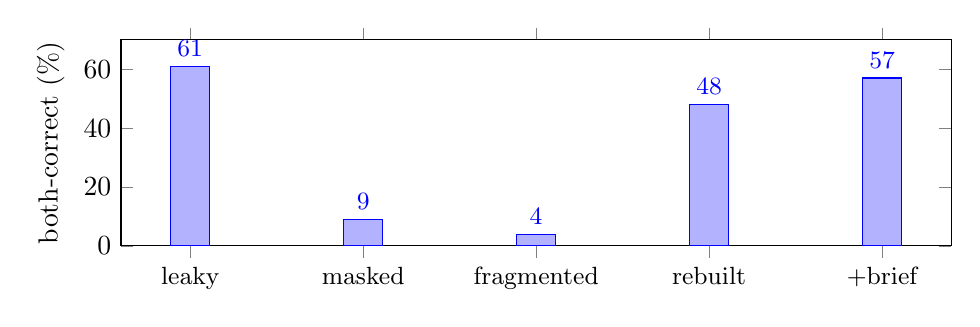
\begin{tikzpicture}
\begin{axis}[width=\columnwidth, height=4.2cm, ybar, bar width=14pt,
  ylabel={both-correct (\%)}, ymin=0, ymax=70, ytick={0,20,40,60},
  symbolic x coords={leaky, masked, fragmented, rebuilt, +brief},
  xtick=data, x tick label style={font=\small}, nodes near coords,
  every node near coord/.append style={font=\small}]
\addplot coordinates {(leaky,61) (masked,9) (fragmented,4) (rebuilt,48) (+brief,57)};
\end{axis}
\end{tikzpicture}
\caption{The honesty arc (both-correct on identical incidents): removing leaks
collapses performance; rebuilding generic evidence recovers --- and on localization
exceeds --- it.}
\label{fig:honesty}
\end{figure}

\subsection{RQ-C: What is kernel telemetry worth?}
\label{sec:results-kernel}

\begin{table}[t]
\caption{Kernel-tier ablation (23 incidents $\times$ 4 tiers; brief on, skills off).}
\label{tab:kernel}
\begin{tabular}{lcccc}
\toprule
Kernel view & Service & Fault & Both & Agent calls \\
\midrule
L1+L2+L3 & 83\% & 61\% & 61\% & \textbf{9.1} \\
L1 only & 74\% & 48\% & \textbf{43\%} & 10.1 \\
L3 only & 78\% & 57\% & 57\% & 10.0 \\
none & 78\% & 57\% & 57\% & 12.2 \\
\bottomrule
\end{tabular}
\end{table}

\textbf{K1.} Removing kernel telemetry entirely costs $\le$4 points (within the noise
band) but $+34\%$ investigation effort: with strong cross-modality tooling, kernel's
robust value at full telemetry is \emph{efficiency}, not rescue. \textbf{K2.} The one
stable loss is induced-DB-latency \emph{typing}: wait attribution converts ``the
datastore is the locus'' into ``induced latency, not an application bug''.
\textbf{K3.} \emph{A partial kernel view is worse than none}: raw KPIs without
interpretive framing send the agent chasing kernel noise ($-14$ points vs.\
kernel-blind; four families lost, none gained) --- representation quality dominates
kernel presence. \textbf{K4.} The pre-registered hypothesis that removing kernel
causes the largest drop on blind-spot faults is \emph{not confirmed at full
telemetry}: kernel-decisive families hold 85\% service in every tier because our
limit-signal/topology/host tools absorbed the signal (recorded in the
pre-registration amendment log). The interaction test sharpens this
(\S\ref{sec:results-interact}): the kernel advantage does not grow under trace
\emph{thinning} either --- but kernel \emph{does} compensate under complete trace
\emph{removal}, restoring both locus and typing on induced DB latency. H2 is thereby
refined rather than merely refuted: kernel is a compensating channel under modality
loss, not under modality thinning. Behaviorally, the kernel-blind agent wastes
${\sim}30\%$ of calls re-probing the empty modality unless the tool answers
definitively once --- an agent-design lesson in its own right.

\subsection{RQ-D: Telemetry degradation --- no cliff on any axis}
\label{sec:results-trace}

\begin{table}[t]
\caption{Degradation axes on the agent (23 incidents per condition; both-correct;
single-run noise band ${\pm}9$ points). Full per-condition tables in the artifact.}
\label{tab:degradation}
\begin{tabular}{llll}
\toprule
Axis & Range tested & Both-correct span & Verdict \\
\midrule
Traces & 100\%$\to$5\% retention & 43--57\% & flat (10\% scores best) \\
Metrics & 5\,s$\to$60\,s scrape & 43--52\% & flat (30\,s scores best) \\
Logs & ALL$\to$ERROR-only & 43--57\% & flat (ERROR beats WARN) \\
Kernel & full ladder$\to$none & 43--61\% & $-4$ pts, $+34\%$ calls; L1-only worst \\
\bottomrule
\end{tabular}
\end{table}

\paragraph{Traces.} Across 100/50/25/10/5\% whole-trace retention (115 diagnoses),
both-correct stays within 43--57\% (the noise band; 10\% retention scores best), 18/23
incidents produce identical outcomes at every level, and the tool mix is constant.
Mechanism: the agent consumes spans as \emph{aggregates} --- brief latency tops and
topology edge percentiles --- which survive uniform sampling; direct raw-trace reads
are nearly absent. The baselines were flat because they never extracted trace value;
the agent is flat because its trace use is statistical and redundantly backed --- the
same curve for the opposite reason. \emph{Implication: ${\sim}20\times$ trace
collection-cost reduction without diagnostic loss} at otherwise-full telemetry.

\paragraph{Metrics.} Coarsening scrape resolution 5$\to$60\,s (92 diagnoses) moves
both-correct 43/48/52/48\% --- non-monotonic, with 30\,s scoring best, and per-family
flips balanced in both directions (pure churn). The tools compute window-level rates
and means over 60--120\,s windows; a counter needs only two samples per window, so
even 60\,s scrape preserves every delta the agent reads.

\paragraph{Logs.} Filtering ALL$\to$WARN$\to$ERROR-only (69 diagnoses) gives
57/43/52\% --- ERROR-only \emph{beats} WARN, confirming non-signal: the log tool keys
on error-class signature \emph{changes}, which survive the harshest filter by
construction. The one incident recurring in loss lists across both axes (Sock~Shop
memory-cap) is also in the A/A flip-prone set, so we make no per-family claim.

\begin{figure}[t]
\centering
\begin{tikzpicture}
\begin{axis}[width=\columnwidth, height=4.6cm,
  xlabel={degradation severity (normalized: 0 = full telemetry)},
  ylabel={both-correct (\%)}, ymin=0, ymax=70, ytick={0,20,40,60},
  xmin=-0.03, xmax=1.03, legend style={font=\scriptsize, at={(0.02,0.02)},
  anchor=south west, legend columns=2}, grid=major, grid style={dashed,gray!25}]
% noise band around the full-telemetry reference (57 +/- 9)
\addplot[draw=none, fill=gray!15, forget plot] coordinates
  {(-0.03,48) (1.03,48) (1.03,66) (-0.03,66)} \closedcycle;
\addplot+[mark=*] coordinates {(0,52) (0.25,52) (0.5,43) (0.75,57) (1,43)};
\addlegendentry{traces 100$\to$5\%}
\addplot+[mark=square*] coordinates {(0,43) (0.33,48) (0.67,52) (1,48)};
\addlegendentry{metrics 5$\to$60\,s}
\addplot+[mark=triangle*] coordinates {(0,57) (0.5,43) (1,52)};
\addlegendentry{logs ALL$\to$ERROR}
\addplot+[mark=diamond*] coordinates {(0,61) (0.33,43) (0.67,57) (1,57)};
\addlegendentry{kernel full$\to$none}
\end{axis}
\end{tikzpicture}
\caption{Both-correct under per-axis degradation (23 incidents per point; shaded band
= single-run noise around the full-telemetry reference). No axis exhibits a cliff;
the kernel dip at severity 0.33 is the L1-only tier (partial view worse than none).}
\label{fig:degradation}
\end{figure}

\paragraph{Consolidated RQ-D answer.} There is no degradation cliff at standard
operational ranges (Table~\ref{tab:degradation}, Fig.~\ref{fig:degradation}). The pre-registered cliff expectation
resolves as a \emph{robustness} result with one structural cause: the agent consumes
every modality at the aggregate level, with evidence redundant across modalities ---
when one channel thins, the fault signature usually survives in another. The one real
hazard is qualitative, not quantitative: a \emph{badly represented} modality (raw
kernel KPIs alone, \S\ref{sec:results-kernel}) hurts more than an absent one.
Practically: 5\% traces $+$ 60\,s metrics $+$ ERROR-only logs cost an agentic-RCA
consumer nothing measurable, while kernel telemetry pays via investigation efficiency
and induced-DB-latency typing.

\subsection{RQ-D$'$: Interaction and whole-modality removal}
\label{sec:results-interact}

\paragraph{Kernel $\times$ thinned traces.} At 25\% and 10\% trace retention the
kernel-blind agent matches or exceeds the kernel-full agent (both-correct 48 vs.\ 30\%
at 25\%; 57 vs.\ 57\% at 10\%; kernel-decisive families show no kernel edge at any
retention), while kernel-blindness costs $+1.5$--$2$ calls at every level. The kernel
advantage is retention-\emph{invariant} in accuracy and constant in efficiency ---
there is no compensation effect under thinning. (The 25\%-retention cell is weak in
every sweep containing it: deterministic seeding keeps the same span sample per run,
so one unlucky sample recurs --- a seeding artifact we report rather than average
away.)

\paragraph{Whole-modality removal.} Dropping kernel entirely (78/48/48) replicates
the kernel-none tier through a different code path --- a free A/A check. Dropping
\emph{traces} entirely is the first modality loss that visibly hurts: 70/48/43
($-14$ both) at $+74\%$ investigation effort, with losses concentrated on the
path-shaped Train-Ticket faults whose evidence is topological. The trace no-cliff
result is therefore threshold-like: \emph{aggregates survive any sampling; presence
matters}. And with traces gone, kernel compensation finally appears in its
pre-registered direction: Sock~Shop induced-DB-latency stays fully correct on kernel
wait-attribution alone. Either modality suffices to localize the datastore; kernel is
required for typing; only losing both would break the case. Behaviorally, the
no-traces agent spent ${\sim}37\%$ of calls on the two dead tools --- the
definitive-unavailable answer (\S\ref{sec:results-kernel}) should generalize to every
modality.

\subsection{RQ-E: How the investigation itself changes}
\label{sec:results-behavior}

Every diagnosis carries its full trajectory, giving degradation a behavioral
signature to accompany the accuracy curves:

\emph{No escalation under thinning.} Across trace, metric, and log thinning the tool
mix is essentially constant --- the agent does not switch strategies because nothing
it relies on was lost (its consumption is aggregate-level throughout).

\emph{Broad-front widening under loss.} When a modality is \emph{removed}, every
remaining tool's usage rises together (kernel-blind: logs $+67\%$, topology $+32\%$,
metrics $+22\%$; trace-blind: all channels up, $+74\%$ total calls) --- compensation
is diversified rather than a single substitute channel.

\emph{Effort is a leading indicator.} Tool-call counts rise \emph{before} accuracy
falls: kernel removal costs $+34\%$ calls at $-4$ points; trace removal $+74\%$ calls
at $-14$. In an operational deployment, investigation effort is an earlier signal of
telemetry inadequacy than accuracy, which is only observable with ground truth.

\emph{Dead-modality thrashing.} Absent a definitive ``unavailable'' tool answer, the
agent re-probes empty modalities per-service: ${\sim}30\%$ of calls under
kernel-none, ${\sim}37\%$ under trace-removal went to empty tools. A one-line tool
change eliminates the former; we report the latter unfixed for internal consistency
of the sweep.

\subsection{RQ-F: Does an experience (skills) layer help?}
\label{sec:results-skills}

\begin{table}[t]
\caption{Skill-library conditions (23 incidents each; masked; selector sees only the
evidence digest and may abstain).}
\label{tab:skills}
\begin{tabular}{lccc}
\toprule
Condition & Service & Fault & Both \\
\midrule
No skills (floor) & 83\% & 57\% & 57\% \\
+ context brief (config of record) & \textbf{87\%} & \textbf{61\%} & 57\% \\
+ full skill library & 78\% & 43\% & 43\% \\
Leave-one-family-out (unseen fault) & 70\% & 39\% & 39\% \\
\bottomrule
\end{tabular}
\end{table}

The deterministic Context Builder is the clear win: equal-or-better accuracy at
$-41\%$ calls and $-58\%$ input tokens. Skills lift individual families (co-tenant
contention is solved \emph{only} with its skill; cap-fault typing improves) but
mis-selection --- concentrated on the shared-datastore application, where background
DB edges attract db-flavored skills --- costs more than skills contribute (selection
15/23). Under leave-one-family-out the selector almost never abstains (1--3/23);
distractor skills cost ${\sim}18$ points vs.\ the skill-free floor, though the agent's
ability to override a wrong skill caps the damage (19/23 cells unchanged).
\emph{Experience layers require selection quality before they are safe on
out-of-library incidents.} We release the full selection-confusion data.

\subsection{RQ-G: The minimum observability budget}
\label{sec:results-budget}

\begin{table}[t]
\caption{Budget configurations (23 incidents each). ``MB touched'' = telemetry the
tools actually consumed per incident; reduction is vs.\ the full-telemetry
configuration of record.}
\label{tab:budget}
\begin{tabular}{lccccc}
\toprule
Configuration & Service & Both & Calls & MB touched & Reduction \\
\midrule
Full (config of record) & 83--87\% & 48--57\% & 9.0 & 1390 & 1$\times$ \\
Lean (5\% traces, 60\,s, ERROR) & 78\% & 43\% & 7.6 & 24.5 & \textbf{57$\times$} \\
Minimal (lean $-$ kernel) & 83\% & 39\% & 11.0 & 12.1 & 115$\times$ \\
\bottomrule
\end{tabular}
\end{table}

Each cheap setting is individually free (\S\ref{sec:results-trace}); RQ-G asks whether
they are free \emph{together}. Largely, yes (Table~\ref{tab:budget}): the lean
configuration touches \textbf{57$\times$ less telemetry} while retaining
${\ge}90\%$ of full localization (78\% vs.\ 83--87\%) and both-correct at the lower
edge of the single-run band (43\% vs.\ the 48--57\% A/A range) --- \emph{fault
typing, not localization, is the budget-sensitive component}. Removing kernel as well
(115$\times$) leaves localization intact (83\%) but costs typing further (39\%) and
raises effort ($+45\%$ calls), consistent with kernel's efficiency-and-typing role
throughout. Per-incident LLM cost falls to \$0.009 at 7.6 calls under lean. The
Pareto frontier over all measured configurations is therefore: \emph{minimal} for
cheapest localization, \emph{lean} for balanced budget, \emph{full} only when fault
typing matters --- and since the agent consumes derived kernel views (megabytes),
never raw L0, the kernel term of the budget is collection overhead ($-0.5$\%
throughput, \S\ref{sec:dataset}) rather than storage. One incidental observation:
Train-Ticket induced-DB-latency, unsolved at full telemetry in this pass, becomes
fully correct under lean --- thinner traces can \emph{reduce} distraction on
borderline incidents (per-family map: Appendix~\ref{sec:appendix-families}).

\section{Discussion}
\label{sec:discussion}

\paragraph{For benchmark authors.} Injected-fault benchmarks leak by construction ---
through identifiers, not train/test overlap. Masking must preserve cross-tool identity
or it destroys legitimate evidence along with the hints. Scores alone are
unverifiable; publish transcripts and an executable auditor with them.

\paragraph{For agent builders.} Representation beats raw access: interpreted kernel
summaries outperform raw KPIs, and a partial view can be worse than none
(\S\ref{sec:results-kernel}). Tools should answer \emph{definitively} when a modality
is absent, or the agent thrashes on it. A deterministic context builder bought more
accuracy-per-dollar than any prompt refinement we attempted.

\paragraph{For observability practice.} At otherwise-full stacks, 5\% whole-trace
sampling appears safe for LLM-agent RCA --- a ${\sim}20\times$ collection saving on
the most instrumentation-expensive modality. Kernel tracing costs $-0.5$\% throughput
to collect and repays $-25$\% agent effort to use, while uniquely supplying
induced-DB-latency typing.

\paragraph{Label semantics vs.\ mechanism.} A closed fault taxonomy penalizes
mechanically correct explanations (connection-reset storms described accurately but
labeled as outages). We report label-strict scores and release evidence text to enable
mechanism-level judgment. \todo{mechanism-correct secondary metric}

\section{Threats to Validity}
\label{sec:threats}

\paragraph{Internal.} Single-run condition aggregates carry a measured $\pm{\sim}9$
point band; we report it explicitly, repeat borderline incidents ($r{=}3$), and prefer
per-family flip evidence over headline deltas. The injection window doubles as alert
time for all methods equally.

\paragraph{External.} One LLM (GPT-5.4) --- the harness is multi-provider but
cross-model replication remains \todo{run}; two subject systems (chosen for
architectural contrast); injected rather than organic faults; agent sweeps use the
23-incident gate (93 incidents available) for cost control.

\paragraph{Construct.} The closed fault taxonomy penalizes mechanism-correct
diagnoses at label boundaries (\S\ref{sec:discussion}); trace degradation so far uses
uniform whole-trace sampling, the gentlest regime --- cliffs may exist under harsher
transforms. Masking asymmetry favors the \emph{baselines} (the statistical baseline
still exploits container names), making our agent-vs-baseline comparison conservative.

\section{Conclusion}
\label{sec:conclusion}

We asked how much an LLM RCA agent's reported skill survives honest evaluation, and
how much observability it actually needs. The answers: naming leaks alone were worth
57~points of fault-classification accuracy; with leaks closed, generic cross-modality
tooling still roughly doubles non-LLM baselines on localization at a cent per
incident; traces are ${\sim}20\times$ over-collected for this task --- degradation by
\emph{thinning} costs nothing on any axis, while degradation by \emph{loss} is where
modalities earn their keep (removing traces costs 14~points and 74\% more effort;
kernel then steps in as the compensating channel, alone recovering induced-DB-latency
end to end); kernel telemetry is otherwise an efficiency multiplier and the sole
source of induced-DB-latency typing, but only in \emph{interpreted} form --- raw
kernel numbers are worse than none; and experience layers help only as far as their
selection is reliable. All claims ship with machine-checkable no-leakage certificates
over 600+ transcripts.

\todo{final data-availability sentence with DOI}


\appendix
\section*{Appendix: outcome per fault type across key setups}
\label{sec:appendix-families}

\newcommand{\Yes}{$\bullet$}
\newcommand{\Svc}{$\circ$}
\newcommand{\No}{--}

$\bullet$ = component and fault type both right; $\circ$ = right component only;
-- = miss. Columns: our standard setup (with the evidence briefing); kernel given in
full / as raw numbers only / absent; traces removed entirely; the lean and minimal
budget setups. S = Sock Shop, T = Train Ticket. Generated directly from the recorded
results by the released analysis scripts.

\begin{table}[h]
\centering
\small
\begin{tabular}{lccccccc}
\toprule
Fault (application) & standard & kernel full & kernel raw & no kernel & no traces & lean & minimal \\
\midrule
Host CPU overload (S) & \Yes & \Yes & \Yes & \Yes & \Yes & \Yes & \Yes \\
Host disk overload (S) & \Yes & \Yes & \Yes & \Yes & \Yes & \Yes & \Yes \\
Host memory exhaustion (S) & \Yes & \Yes & \Yes & \Yes & \Yes & \Svc & \Svc \\
Host network degradation (S) & \No & \No & \No & \No & \No & \No & \No \\
Frozen dependency (S) & \Yes & \Yes & \Yes & \Yes & \Yes & \Yes & \Yes \\
Error burst (S) & \Svc & \Svc & \Svc & \Svc & \Svc & \Svc & \Svc \\
Noisy neighbour (S) & \Svc & \Yes & \Svc & \Yes & \Svc & \Svc & \Yes \\
Silent queue backlog (S) & \No & \No & \No & \No & \No & \Svc & \No \\
Slow database (S) & \Yes & \Yes & \Yes & \Svc & \Yes & \Yes & \Svc \\
Service CPU limit (S) & \Yes & \Yes & \Yes & \Yes & \Yes & \Yes & \Yes \\
Service memory cap (S) & \Svc & \Yes & \Svc & \Yes & \Svc & \No & \No \\
Single-service network fault (S) & \Svc & \Svc & \No & \Svc & \No & \Svc & \Svc \\
Host CPU overload (T) & \Yes & \Yes & \Yes & \Yes & \Yes & \Yes & \Yes \\
Host disk overload (T) & \Yes & \Yes & \Yes & \Yes & \Yes & \Yes & \Yes \\
Host memory exhaustion (T) & \Yes & \Yes & \Yes & \Yes & \Yes & \Yes & \Yes \\
Host network degradation (T) & \Svc & \Svc & \Svc & \No & \Svc & \Svc & \Svc \\
Frozen dependency (T) & \Yes & \Yes & \No & \Yes & \No & \No & \No \\
Error burst (T) & \Svc & \Svc & \Svc & \Svc & \Svc & \Svc & \Svc \\
Noisy neighbour (T) & \Svc & \Svc & \Svc & \Svc & \Yes & \Yes & \Svc \\
Slow database (T) & \No & \No & \No & \No & \No & \Yes & \Svc \\
Service CPU limit (T) & \Yes & \Yes & \Yes & \Yes & \No & \No & \Yes \\
Service memory cap (T) & \Svc & \No & \Svc & \No & \Svc & \Svc & \Svc \\
Single-service network fault (T) & \No & \Yes & \No & \Yes & \No & \No & \Svc \\
\bottomrule
\end{tabular}
\end{table}


\bibliographystyle{ACM-Reference-Format}
\bibliography{references}

\end{document}
